\documentclass{suribt}
\title{ゲーム「2048」のプレイヤについて}
\author{金澤望生}
\eauthor{Kanazawa Nozomu}
\studentid{08-152021}
\supervisor{山口和紀 教授}
\handin{2018}{1}
\keywords{2048,パズルゲーム,強化学習,ヒューリスティクス}
\usepackage[dvipdfmx]{graphicx}
\usepackage{float}
\usepackage{algorithm}
\usepackage{algorithmic}
\usepackage{amsmath}
\usepackage{array}

\makeatletter
\newenvironment{breakablealgorithm}
  {% \begin{breakablealgorithm}
   \begin{center}
     \refstepcounter{algorithm}% New algorithm
     \hrule height.8pt depth0pt \kern2pt% \@fs@pre for \@fs@ruled
     \renewcommand{\caption}[2][\relax]{% Make a new \caption
       {\raggedright\textbf{\ALG@name~\thealgorithm} ##2\par}%
       \ifx\relax##1\relax % #1 is \relax
         \addcontentsline{loa}{algorithm}{\protect\numberline{\thealgorithm}##2}%
       \else % #1 is not \relax
         \addcontentsline{loa}{algorithm}{\protect\numberline{\thealgorithm}##1}%
       \fi
       \kern2pt\hrule\kern2pt
     }
  }{% \end{breakablealgorithm}
     \kern2pt\hrule\relax% \@fs@post for \@fs@ruled
   \end{center}
  }
\makeatother

\begin{document}
\maketitle

\frontmatter
\begin{abstract}
インターネットブラウザやスマートフォン上で遊ぶことのできるパズルゲーム「2048」は2014年3月に公開されて以来世界中で人気を博すパズルゲームとなったが,これにはルールが直感的で理解しやすい一方でその攻略法を会得することが難しいという2048特有の性質によるところが大きい.この性質により2048はゲームAI研究の題材としても多く取り上げられ,特に強化学習を用いて訓練したプレイヤがSzubert \& Ja\'{s}kowskiなど多くの研究者によって発表された.しかしながら,これらのプレイヤには人間が2048を遊ぶ際に用いる経験的な知見は盛り込まれておらず,また強化学習によって必ずしも学習できているとは言えない方策も存在している.本研究においては,特に人間が2048を遊ぶ際に大きなタイルを隅に寄せる傾向があることに注目し,これを「maxtile-in-corner方策」と名付け,既存研究による強化学習ベースのプレイヤに組み込んだ.その結果,maxtile-in-corner方策を組み込んだプレイヤは既存の強化学習で訓練したのみのプレイヤよりも有意に優れた指標を残し,強化学習だけでは習得できない人間の経験的な知見をAIプレイヤにトップダウン的に適用することの効果を示した.
\end{abstract}

\tableofcontents

\mainmatter
\chapter{導入}
本章においては,2048を本研究の題材として採用した動機付けを述べるとともに,2048というゲームのあらましやルールについて説明し,次章以降の展開に対する準備を行う.

\section{モチベーション}
「2048」\cite{2048game}は,インターネットブラウザおよびスマートフォンなどの端末でプレイすることができるパズルゲームである.非常にシンプルで誰もが直感的にルールを理解できるのに対し,ゲームを理解したり安定して勝ち続けたりすることは非常に難しい\cite{Szubert}2048は,その絶妙なバランスが評価されて非常に多くの人々が遊ぶようになった.同時に2048はゲームAI研究の対象としても活発に取り上げられるようになり,近年では強化学習を用いて訓練した非常に強いプレイヤが複数の研究者から発表されている\cite{Szubert}\cite{Wu}\cite{Oka}\cite{Yeh}\cite{Jaskowski}.

これらのプレイヤの実装手法は汎用性が高く,他のゲーム(特に2048に類似したゲーム)や課題に対しても適用することが可能な手法が多く用いられている\cite{Yeh}反面,人間が2048をプレイする際に用いている経験的な知識・方策は明示的に組み込まれていないことが多い.一部の先行研究においては特徴量として人間が注目する指標を組み込んでいる\cite{Yeh}ものの,これらの指標も強化学習によって訓練されるため,経験的な知識が学習によって獲得されるとは言い難い.

\section{本研究の目的}
本研究においては,これまでに発表されてきた強化学習で訓練を行う2048プレイヤに対して,人間による経験的な知識に基づく新たなヒューリスティックスを導入する.このヒューリスティックスは強化学習による価値関数とは独立に組み込み,強化学習によって訓練された学習器を補助する形で適用することにする.新たなヒューリスティックスを導入した結果,ヒューリスティックスを導入していない2048プレイヤよりも,導入したプレイヤの方が良い性能を示すことを明らかにするのが,本研究の目的である.

\section{2048について}
2048がGabriele CirulliによってGitHub上に公開されたのは2014年3月のことである\cite{BusinessInsider}.Cirulliは2048を開発していた当時,「1024」および「2048」\footnote{Cirulli自身が発表した2048とは似ているが,ルールが異なる別のゲームである}というゲームに熱中していた\cite{CirulliMedium}.これらのゲームはどちらもAsher Vollmerによるゲーム「Threes」にルールがよく似ている類似作品であるが,Cirulliは当時Threesの存在については認識していなかった.CirulliはこれらのThreesに端を発するゲームを改良するべく新たなゲームを開発し,ついに「2048」として公開することとなった.ここで挙げた1024,Cirulliが参考にした2048,そしてCirulli自身が発表した2048は全てThreesの類似作品であるものの,これらの作品群の中ではCirulliによる2048が最も人気を集めており,全世界で2300万人以上の人が2048\footnote{なお,ここから単に2048と表記した場合,それはCirulliが開発した2048のことを指す}で遊んだとされる\cite{CirulliMedium}.

2048はシンプルで直感的にルールを理解できる一方で,マスターすることが非常に難しいゲームであることが特徴となっており,このために多くのプレイヤーを熱中させていると同時にゲームAI研究の題材としても多く取り上げられていると考えられる.また,ゲームとしての2048について着目すると,2048については以下のような特徴を挙げることができる:

\subsubsection{完全情報ゲームである}
2048は単一の状態から始まり,1人のプレイヤが自分の手番で何かしらの行動を起こすことによって状態が遷移し,さらにプレイヤはゲームの状態を全て把握することができる.したがって,2048は完全情報ゲームであると言える.

\subsubsection{非決定論的ゲームである}
2048は1人のプレイヤによってのみプレイされるゲームであるが,状態の変化の際には乱数によって決定される要素があるため,プレイヤは次の状態を知ることはできない.したがって,2048は非決定論的(nondeterminisitc)ゲームである.ただし,プレイヤは次の状態がいくつあり,その状態にどれぐらいの確率で遷移するのか自分で計算することはできる.

\subsubsection{明確な終局が予め設定されていない}
チェスや将棋といったゲームについては,どのような状態に到達するとゲームが終了するのか規定されており,プレイヤはお互いに相手を終局に向かわせることを念頭にゲームをプレイする.一方で,2048には次の状態に遷移することが不可能になったらゲームが終了するというルールはあるものの,その状態に到達するまでは無限にゲームを進めることができる.すなわち,プレイヤが熟達すればするほど長い時間ゲームを進めることができ,その分プレイヤの優秀さを示す指標も良くなる.この特徴により,2048は強化学習やゲームAIのベンチマークとしてよく機能していると考えられる.

\section{2048のルール}
\subsection{用語定義}
\subsubsection{盤面}
2048を遊ぶのに用いる大きな土台のことで,$4 \times 4 = 16$個の\textbf{マス}が正方形をなすように並べられている.1つのマスは,空であるか,1個の\textbf{タイル}が入っているかのどちらかである.1個のタイルには$2^n (n>0)$の数1つが書かれている.また,盤面を囲んでいる4辺のことを盤面の\textbf{終端}と呼ぶことにする.

\subsubsection{初期盤面(\textit{initial state})}
プレイヤが2048のゲームを始める時には,必ず初期盤面を与えられる.初期盤面とは,全てのマスにタイルが入っていない状態の盤面に対して,2個のランダムタイル(後述)が与えられた盤面のことである.ランダムタイルがどの位置に発生するかはそのゲームを始めるまで分からないため,プレイヤはゲームごとに異なる初期盤面を与えられ,なおかつその初期盤面を予想・決定することはできない.

\subsubsection{終末盤面(\textit{terminal state})}
プレイヤが2048のゲームを進めた結果,空のマスが1つもなく,なおかつ後述する\textbf{アクション選択}が行えない盤面に到達したなら,ゲームを終了する.この時の盤面を終末盤面とする.

\subsubsection{${\nu}$-タイル}
${\nu}$という数が書かれたタイルのことを${\nu}$-タイルと呼ぶことにする.

\subsubsection{ランダムタイル}
2048のゲームを遊ぶ中で,ランダムタイルと呼ばれる新しいタイルが盤面に追加されることがある.ランダムタイルは盤面上の空のマスのどこかに追加される.なお,空のマスが存在しない盤面に対してランダムタイルが追加されるような状況は,2048のゲーム中に存在しない.ランダムタイルは2-タイルもしくは4-タイルであり,2-タイルが追加される確率は0.9,4-タイルが追加される確率は0.1と定められている.ランダムタイルが追加されるマスの位置はランダムに決定される.

\subsubsection{報酬(\textit{reward})とスコア}
2048における報酬とは,プレイ後の\textbf{報酬加算}の手順で加算される数値のことを指す.また,ゲームが終了するまでに加算された報酬の総和を\textbf{スコア}と呼ぶ.

\subsubsection{プレイ}
本研究において,\textbf{プレイ}という用語を以下のように定義する:
\begin{itemize}
\item プレイヤは,自分の手番1回につき,1回のプレイを行うことができる.
\item 1回のプレイは,\textbf{アクション選択},\textbf{遷移},\textbf{ランダムタイル生成}の3つの手順からなる.
\item プレイヤは,1回のプレイの間,アクション選択を行うことで盤面を操作することができる.なお,プレイヤはアクション選択の結果行われる遷移の後どのような盤面になるのか計算して求めることはできるが,ランダムタイル生成後にどのような盤面になるかを知ることはできない(確率的に予想することはできる).
\end{itemize}

\subsection{ゲームとプレイヤ評価の流れ}
2048において,以下の手順を「1ゲーム」と数える.

\begin{enumerate}
\item ゲームを開始する.プレイヤは初期盤面を与えられる.ゲーム開始時のスコアは0である.
\item プレイを行う.プレイは次の3つの手順からなる:
	\begin{enumerate}
	\item \textbf{アクション選択}:盤面上の全てのタイルを動かす方向を,上下左右のうちいずれかから選ぶ.ただし,次の手順で遷移を行っても盤面に変化が生じないようなアクションを選ぶことはできない.
	\item \textbf{遷移}:盤面上の全てのタイルを,選択したアクションの方向へ,他のタイルもしくは終端に接触するまで動かす.もし任意の${\nu}$-タイル2つが接触したならば,\textbf{マージ}を行う.マージを行ってもなお,アクションの方向へ動かすことができるタイルがあるならば,さらに他のタイルか終端に接触するまで動かす.
	\begin{itemize}
		\item \textbf{マージ}:アクションの方向に向かって前方のタイルを$2{\nu}$-タイルに変更し,後方のタイルを削除する.値が変更された$2{\nu}$-タイルはこの遷移中二度とマージを行わない.同一列において複数組のマージできるタイルがあるならば,マージは前方のタイルを優先して順番に行う.
		\item \textbf{報酬加算}:プレイ中にマージが発生した結果,新たに盤面に$2{\nu}$-タイルが発生したならば,$2{\nu}$を報酬としてスコアに加算する.報酬加算はマージを行った結果新たに発生した全てのタイルについて行う.
	\end{itemize}
	\item \textbf{ランダムタイル生成}:1個のランダムタイルを盤面上に生成する.
	\end{enumerate}
\item 1回のプレイが終末盤面に到達することなく終了したならば,次のプレイを行う.もし遷移もしくはランダムタイル生成の手順において終末盤面に到達したならば,ゲームを終了する.
\end{enumerate}

\subsection{2048で重要な指標}
\subsubsection{$max tile$}
ゲームが終末盤面に到達した時点で,盤面上で最も大きな数のタイルを$max tile$と呼ぶ.近年の2048プレイヤの研究の多くは16384-タイルの作成に成功しており,32768-タイルの作成に成功したプレイヤもある\cite{Jaskowski}.32768を達成することが2048のプレイヤ実装において大きなメルクマールとなることから,32768-タイルを作成できた割合を指標とすることもある\cite{Jaskowski}.

\subsubsection{勝率}
2048において,$max tile \geq 2048$ならば,プレイヤーの勝利であると定義されている.多くの研究が90\%以上の勝率を達成しているが,ゲーム木探索を組み合わせたプレイヤは勝率は100\%を達成しており,勝率については問題にしないこともある.

\subsubsection{スコア}
2048において最も重要な指標がスコアである.プレイヤの学習が終わった後にその性能を検証するゲームを何度か行った際,その検証中のスコアの算術平均を取った\textbf{平均スコア}と,その検証中に最も高かったスコアである\textbf{最高スコア}の2つが,プレイヤの性能を示す指標として用いられることが多い.

\subsection{2048プレイヤの学習に関する用語定義}
\subsubsection{学習ゲーム}
プレイヤを訓練するために行うゲームのことで,価値関数などのパラメータの更新を行いながらゲームを進める.ゲームを開始してから終末盤面に到達するまでを1ゲームと数え,1ゲームが終了したら次の学習ゲームに進む.後述する通り,学習ゲームをどれくらい行うかについては実験者が指定する.一般的に学習ゲームを多く行えば行うほど学習器の性能は良くなるが,特定の状況に特化して学習を行う過学習を引き起こす可能性もある\cite{Yeh}.

\subsubsection{検証ゲーム}
訓練されたプレイヤを用いてゲームを行う.この際,価値関数などのパラメータは参照するだけで更新は行わない.1回の実験において,学習ゲームを行う回数$n$と,学習中に検証ゲームを行うインターバルのゲーム数$i$と,検証ゲームを行う回数$m$は実験者が指定する.$i,m$については,本研究および先行研究においては$i=5000, m=1000$と指定されている.$n$については研究により左右するが,1回の実験あたり100,000ゲームか,500,000ゲームか,もしくは1,000,000ゲームの学習ゲームを行うようになっている.本研究では$n=500000$もしくは$n=1000000$としている.

\chapter{先行研究}
この章では,2048プレイヤを実装した先行研究について,その研究が用いた手法と実装されたプレイヤの成績について紹介する.

\section{Szubert \& Ja\'{s}kowski (2014)}
Szubert \& Ja\'{s}kowskiは,強化学習の手法の1つであるTD学習を用いたプレイヤの訓練とnタプルネットワークを用いた価値関数\footnote{本研究および先行研究における価値関数(value function)とは,2048の盤面全体の集合$S$からその盤面の評価値を示す数値$W$への写像$V: S \rightarrow W$であり,$V(s)$はルックアップテーブルなどに保持されている盤面$s$の評価値を\textbf{参照して}その値を返す.盤面の状況をもとにその評価値を\textbf{計算して}値を返す評価関数(evaluation function)とは異なる}の表現を組み合わせることによって,人間の知識やゲーム木探索を使用しないで十分強い2048プレイヤを実装することに成功した.

\subsection{TD学習}
TD学習の「TD」とは\emph{temporal difference}の略であり,すなわち状態間における価値の差分を学習することによって価値関数$V(s)$の訓練を行う手法である.TD学習はTesauroによるバックギャモンへの適用\cite{Tesauro}でよく知られるようになり,碁\cite{Runarsson}\cite{Schraudolph}やオセロ\cite{Dries}\cite{SzubertOthello},チェス\cite{Baxter}におけるゲームAIの方策決定の手法として用いられるようになった.2048にあてはめると,盤面$s$の評価値と,その盤面の1プレイ後の盤面$s''$の評価値の差分を取り,これを現状定まっている$s$の評価値に足し込んでいくことで価値関数の更新を行うことになる.2048プレイヤに対してTD学習を適用する方法はさまざまなものがあるが,Szubert \& Ja\'{s}kowskiが検討した適用の方法は以下の通りである:

\subsubsection{アクションの評価(Q学習)}
平易な価値関数の実装として最初に考えられるのが,アクション$a$を選択した時の盤面$s$の価値を評価する関数$Q(s,a)$を学習する\textbf{Q学習}である.Q学習において,行動評価値$Q(s,a)$は以下のように更新される:

\[
	Q(s,a) \leftarrow Q(s,a) + {\alpha} (r + \max_{a' \in A(s'')} Q(s'', a') - Q(s,a))
\]

ここで,$r$は盤面$s$においてアクション$a$を選択したことにより得られた報酬,$s''$は盤面$s$においてプレイを行った後の盤面,$A(s)$は盤面$s$において選択可能なアクションの集合である.このQ学習においては,プレイ後の盤面$s''$における最も高い行動評価値と報酬の和と,現在の盤面$s$においてアクション$a$を選択することの行動評価値の差を取り,学習率${\alpha}$を掛けて$Q(s,a)$に足し込むという形で,行動価値関数の更新を行っている.

なお2048にQ学習を適用する場合は,どの盤面に対しても有り得るアクションは高々4つしかないので,$s$と$a$の組み合わせにより値を与える1つの関数を使用するのではなく,4通りのアクションごとに価値関数$V_a(s) \;\; (a \in \text{\{\textsc{Up, Down, Right, Left}\}})$を使用することができる\cite{Szubert}.この場合,アクション$a$に対する行動評価値$V_a(s)$は以下のように更新される:

\[
	V_a(s) \leftarrow V_a(s) + {\alpha} (r + \max_{a' \in A(s'')} V_{a'}(s'') - V_a(s))
\]

\subsubsection{盤面の評価(TD(0))}
次に,TD(0)を利用して盤面$s$の価値を評価する手法が挙げられる.TD(0)は最もシンプルなTD学習のアルゴリズムであり,TD(0)における価値関数$V(s)$は次の式のように更新される:

\[
	V(s) \leftarrow V(s) + \alpha (r + V(s'') - V(s) )
\]

一般に,TD(0)によって制御されるエージェントは$r+V(s'')$を目標とする\cite{Sutton}.したがって,盤面の評価を行う際にはこの値を最大化するようなアクションを選択することになるが,このモデルにおいては$r+V(s'')$の\textbf{期待値}を最大化するようなアクションを選択する.すなわち,ある盤面$s$の価値は以下のように評価され,この値を最大化するアクションを選択することになる:

\[
	R(s,a) + \sum_{s'' \in S''} P(s,a,s'')V(s'')
\]

ここで,$R(s,a)$は盤面$s$においてアクション$a$を選択した際に獲得する報酬を与える関数,$S''$は盤面$s$においてプレイを行った後に有り得る盤面の集合を,$P(s,a,s'')$は盤面$s$においてアクション$a$を選択した後に盤面$s''$が得られる確率を与える関数を表す.

盤面の評価モデルは価値関数として単一の$V(s)$のみを保持していればよいため,4つの価値関数を保持する必要があるアクションの評価モデルに対して優位性がある一方で,1つのアクションを評価する際にそのアクションの結果得られる全てのプレイ後の盤面を求める必要がある.2048では最大で15個の空のマスが存在し,これらのマスに生成されるランダムタイルは2種類で,さらに4方向へのアクションを選択できることから,1回のアクション選択のために最大で120個の盤面を求めなければならない.このため,盤面の評価モデルはアクションの評価モデルと比べて実行速度が非常に遅いプログラムとなってしまう.

\subsubsection{遷移後盤面の評価(TD(0))}
最後に提案されたのが,アクションの評価モデルと盤面の評価モデルの組み合わせとも言える遷移後盤面の評価モデルである.遷移後盤面の評価モデルにおいては,単一の価値関数$V$を用いるが,この価値関数は盤面$s$に対して適用するのではなく,$s$の遷移後の盤面$s'$(\textit{afterstate},すなわち遷移を行った後でランダムタイルを生成する前の盤面)に対して適用する.ランダムタイル生成後ではなく遷移後の盤面ならば1つのアクションに対して高々1個しか存在しないため,計算量を抑えることが可能になる.このモデルにおいては,以下の値を最大化するアクションを選択する.

\[
	R(s,a) + V(T(s,a))
\]

ここで,$T(s,a)$は盤面$s$においてアクション$a$を選択した際に遷移した後の盤面,すなわち$s'$を与える関数である.また,遷移後盤面の評価モデルにおいては,$V(s)$の更新を連続した2つの遷移後盤面の評価値を用いて行い,以下のように更新されることになる.

\[
	V(s') \leftarrow V(s') + \alpha (r_{next} + V(s'_{next}) - V(s') )
\]

ここで,$s'_{next}$とは$s$の1プレイ後の盤面$s''$の遷移後盤面として最も評価値が高い盤面を,$r_{next}$は$s'_{next}$への遷移によって獲得した報酬を表す.遷移後盤面の評価モデルにおいては,$r_{next}+V(s'_{next})$を目標として学習が行われる.

Szubert \& Ja\'{s}kowskiによる実験の結果,以上の3つのモデルのうち最も性能が良いのは\textbf{遷移後盤面の評価}を行うモデルであった.以降,本研究および先行研究において単にTD学習と表記した場合,それはSzubert \& Ja\'{s}kowskiが実装したTD(0)による遷移後盤面の評価モデルのことを指すこととする.

\subsection{nタプルネットワーク}
TD学習によって盤面の評価とその学習を行うことができるが,盤面と評価値をどのように結びつけるかが問題になる.まず,2048で有り得るすべての盤面に対して評価値を与える1対1対応のルックアップテーブル(LUT)を作成することを考えると,2048で有り得る盤面の数は$(4 \times 4)^{18} \approx 4.7 \times 10^{21}$と膨大な数になり,このようなLUTを計算機上で実装することは現実的に不可能である.

そこで,一部のマスの組み合わせによる「タプル」というクラスターを作成し,さらに複数のタプルを組み合わせることで盤面を表現する手法「nタプルネットワーク」を2048に導入することが,Szubert \& Ja\'{s}kowskiによって提案された.たとえば,図\ref{figure_001}のようなnタプルネットワークを実装した場合,1つのゲーム内で保持すべき重みの数は860625であり,全ての有り得る盤面に対するLUTを保持するのに対して非常に少なくて済む.

\begin{figure}[t]
	\begin{center}
	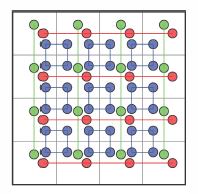
\includegraphics[width=5cm]{figure_001.png}
	\caption{nタプルネットワークの例}
	\label{figure_001}
	\end{center}
\end{figure}

nタプルネットワークはBledsoe \& Browningによりパターン認識に用いられたのが最初の採用例である\cite{Bledsoe}.ゲームAIの分野では,Lucasによってオセロに適用されたことをきっかけに,より広く知られるようになった\cite{Lucas}.

\subsection{結果と課題}
本手法をもとに行った実験のうち,最も良い勝率を達成したプレイヤを用いて10万ゲーム中の成績を検証したところ,勝率は0.9781であり,平均スコアは100,178であった.1ゲーム中に達成されたスコアで最も良かったのは261,526であった.本手法は探索ベースの手法よりも大幅に高速で,かつ成績が良かった\cite{Szubert}.

しかしながら,この手法ではスコアを最大化することを目指して学習を行うため,「常に2048-タイルを生成すること」よりも「時々16384-タイルを生成すること」が重視される傾向があり,したがって勝率は必ずしも100\%を達成できていない.

\section{Wu et al. (2014)}
Wuは,Szubert \& Ja\'{s}kowskiの手法を改良し,木探索を用いた先読みと組み合わせることによってさらに良いプレイヤを実装することに成功した.

\subsection{nタプルネットワークの配置の改善}
Wuは,Szubert \& Ja\'{s}kowskiが考案したnタプルネットワークのうち,直線型で4タプルとして配置していたタプルを,図\ref{figure_002}(b)のように柄杓型の6タプルに変更した.これによって増える重みの数は約2倍程度であったが,この変更によってSzubert \& Ja\'{s}kowskiのものよりも飛躍的に良い成績を得ることができた.なお,何故このようなタプルの配置が最善だと判断したのかについて,Wuは論文において言及していない.

\begin{figure}[t]
	\begin{center}
	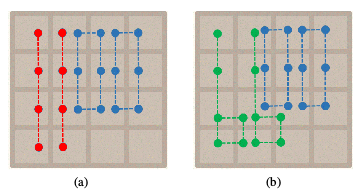
\includegraphics[width=8cm]{figure_002.png}
	\caption{Szubert \& Ja\'{s}kowski(a)とWu(b)が提案したnタプルネットワーク}
	\label{figure_002}
	\end{center}
\end{figure}

\subsection{Multi-Stage TD学習の導入}
Multi-Stage TD学習(MS-TD学習)とは,ゲームのステージ\footnote{本手法においては,盤面に新しい大きな数のタイル(例えば16384-tile)が生成された時を境界として,ゲームをいくつかのステージに分ける}に応じて異なる価値関数を保持することによって,それぞれの局面に対してより適切な重みを学習させることを目的とした手法である.Wuは学習ゲームのそれぞれのゲームを3つのステージに分割し,ゲームプレイも同様に3つのステージに分割して行うようにした.Wuの提案した2048におけるMS-TD学習は,以下のような手順で学習を行う.なお,「$T_{16k}$」とは「その1ゲームの中で初めて16384-タイルを生成することに成功した時」,「$T_{16+8k}$」とは「その1ゲームの中で初めて16384-タイルを生成した後に,初めて8192-タイルを生成することに成功した時」のことを示す.

\begin{enumerate}
\item 第1ステージにおいては,初期盤面からゲームを始めて,価値関数が十分飽和するまで学習を行う.このステージで学習された価値関数の重みのことを「第1ステージ価値関数」と呼ぶことにする.また,学習ゲーム中に$T_{16k}$を達成したなら,その時の盤面を全て保存しておく.
\item 第2ステージにおいては,第1ステージで保存した盤面からゲームを始めて,TD学習を行う.このステージで学習された価値関数の重みのことを「第2ステージ価値関数」と呼ぶことにする.また,学習ゲーム中に$T_{16+8k}$を達成したなら,その時の盤面を全て保存しておく.
\item 第3ステージにおいては,第2ステージで保存した盤面からゲームを始めて,TD学習を行う.このステージで学習された価値関数の重みのことを「第3ステージ価値関数」と呼ぶことにする.
\end{enumerate}

その後,以下のような手順でゲームプレイを行う.

\begin{enumerate}
\item 盤面が$T_{16k}$を達成するまでは,第1ステージ価値関数を用いてゲームプレイを行う.
\item 盤面が$T_{16k}$を達成してから$T_{16+8k}$を達成するまでは,第2ステージ価値関数を用いてゲームプレイを行う.
\item 盤面が$T_{16+8k}$を達成してからは,第3ステージ価値関数を用いてゲームプレイを行う.
\end{enumerate}

\subsection{Expectimax木探索}
Szubert \& Ja\'{s}kowskiによって,木探索ベースの2048プレイヤは強化学習で訓練したプレイヤに劣ることが示されたが,Wuは強化学習によるプレイヤに対してExpectimax木探索を補助的に組み合わせることによって,さらにプレイヤの性能を高めようと試みた.

\begin{figure}[t]
	\begin{center}
	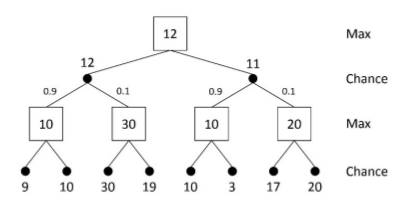
\includegraphics[width=8cm]{figure_003.png}
	\caption{Expectimax木の例 (Wu et al.)}
	\label{figure_003}
	\end{center}
\end{figure}

Expectimax木探索には,MaxノードとChanceノードという2種類のノードがあり,それぞれのノードの値は子ノードから決定される.Maxノードの値は,子ノードのうち最も大きな値のノードの値となる.例えば図\ref{figure_003}の根ノードの値は12であるが,これは子ノードの「12」と「11」のうち最大の値である12を取ったものである.一方でChanceノードの値は子ノードの期待値となる.例えば図\ref{figure_003}の根ノードの子ノードの1つである「12」というノードは,0.9の確率で10となるノードと0.1の確率で3となるノードの期待値,すなわち$0.9 \times 10 + 0.1 \times 3 = 12$によって12という値が決定する.

Wuの提案においては,Maxノードはいわゆる盤面,すなわちこれからプレイヤがアクションを選択して遷移を行おうとする盤面であり,Chanceノードは遷移後盤面,すなわちこれからランダムタイルが発生しようとしている盤面であると考える.例えば,ある盤面(アクション選択と遷移が終わった直後の盤面)の評価値を深さ3のExpectimax木探索を用いて求めたい時,例えば図\ref{figure_010}のような探索木が考えられる.

根ノード$s$はMaxノードであるから,その子ノード(以下,$s'_n \;\; (0 \leq n \leq 3)$と表す)はChanceノードであり,その数は可能なアクションの数$=4$である.根ノードの評価値$V(s)$は$\max\{V(s'_n), 0 \leq n \leq 3\}$である.次に,$s'_0$に注目すると,このChanceノードの子ノード(以下,$s''_m \;\; (0 \leq m \leq 27)$と表す)はMaxノードであり,その数は有り得るランダムタイル生成後の盤面の数$=14 \; \text{(空のマスの数)} \times 2 \; \text{(ランダムタイルの種類の数)} = 28$である.評価値$V(s'_0)$は$V(s''_m)$の期待値で与えられる.さらに$s''_0$に注目すると,このMaxノードの子ノードはChanceノード($s'_{next}$)であり,なおかつ葉ノードである.葉ノードの値は価値関数$V$によって与えられるから,再帰的に親ノードの値も求めることができ,最終的に根ノードの評価値$V(s)$も求められる.

以上のように,Expectimax木の各ノードに盤面を当てはめることによって,任意の深さで先読みをしてから盤面の評価値を求めることが可能であることが示された.Expectimax木探索を用いて先読みをすることで,将来の盤面を予想してより良いアクションを選択できるようになったが,これはスコアの面での成績が良くなることに繋がる一方で,$maxtile=2048$を達成する割合,すなわち勝率の向上にも大きな影響をもたらした.

\begin{figure}[t]
	\begin{center}
	\includegraphics[width=10cm]{figure_010.eps}
	\caption{2048の盤面をExpectimax木に当てはめた例.緑の盤面がMaxノード,青の盤面がChanceノードを表す.}
	\label{figure_010}
	\end{center}
\end{figure}

\subsection{結果と課題}
WuによるプレイヤはSzubert \& Ja\'{s}kowskiのものに比べて著しく良い成績を達成した.まずSzubert \& Ja\'{s}kowskiが達成できなかった32768-タイルの生成に成功し,10.9\%の確率で32768-タイルを生成できるようになった.勝率に関しては1を達成,すなわち2048-タイルは100\%の確率で生成できるようになり,平均スコアは328,946,最大スコアは605,752を記録した.これは当時としては1つの例外\footnote{XiaoによるWuよりも深い先読みと人間による調整を行った評価関数を用いたプレイヤがこの例外であるが,Wuのものよりも100倍遅い:https://www.youtube.com/watch?v=JQut67u8LIg}を除き,当時の計算機による2048プレイヤの中で最も優れた成績であった.

一方で,nタプルネットワークの形状変更やMS-TD学習のステージ分けの方法については,この研究で示された手法が最も良いということを説明する根拠が述べられておらず,依然として改良の余地は残していた.特にnタプルネットワークの形状変更については,次のOka \& Matsuzakiの研究で詳しく検討されることとなった.

\section{Oka \& Matsuzaki (2016)}
Szubert \& Ja\'{s}kowskiは当初図\ref{figure_001}のようなnタプルネットワークを考案していたが,このnタプルネットワークによる学習器はあまり性能が高くなく,平均スコアは10万ゲーム学習した時点で5万〜6万程度にとどまっていた.そこで,図\ref{figure_002}(a)のようなnタプルネットワークへの改良が行われ,その結果平均スコア・勝率ともに改善することができた.さらにWuはSzubet \& Ja\'{s}kowskiの考案したnタプルネットワークを改良し,成績を伸ばすことができた.

しかしながら,ここまでは「タプルのサイズを大きくすると学習器の成績も良くなる」という大まかな関係しかわかっておらず,成績を最善にするnタプルネットワークはどのような形状になるのか厳密には検討されていなかった.これを厳密に検討したのがOka \& Matsuzakiである.

\subsection{nタプル単体の性能の評価}
Oka \& Matsuzakiは,まずnタプル単体の性能を網羅的に評価することを目指した.2048の盤面上でn個のタイルを選んで形成されうるnタプルの数は,表\ref{tab:ntuplesNumber}の通りとなっている\footnote{「Connected」とは,タプル上の全てのタイルが1個以上の他のタプルと隣接していることを示す}.

\begin{table}[t]
	\begin{center}
		\caption{形成されうるnタプルの数}
		\begin{tabular}{l|r|r|r|r|r|r|r|r|r|r|r} \hline
		N & 3 & 4 & 5 & 6 & 7 & 8 & 9 & 10 & 11 & 12 & 13 \\ \hline \hline
		All & 77 & 252 & 567 & 1051 & 1465 & 1674 & 1465 & 1051 & 567 & 252 & 77 \\ \hline
		Connected & 8 & 17 & 33 & 68 & 119 & 195 & 261 & 300 & 257 & 169 & 66 \\ \hline
		\end{tabular}
		\label{tab:ntuplesNumber}
	\end{center}
\end{table}

Oka \& MatsuzakiはConnectedタプルのうち,十分性能が良く,なおかつ現実的にnタプルネットワークとして運用することができる$N=6$と$N=7$の場合のみ検討することとした.彼らは次に,形成されうるConnectedな6タプル68個の中からランダムに10個のタプルを選んで100万ゲームの学習を行う実験を680回\footnote{$680 \times 10 = 6800$より,全てのタプルが100回は選ばれるようにするため}繰り返し,各タプルの性能を比較可能な数値として算出した.7タプルについても同様の実験を行った.

その結果,6タプルと7タプルのうち最も優れた4つのタプルと最も劣った4つのタプルが,図\ref{figure_004}の通り明らかになった.

\begin{figure}[t]
	\begin{center}
	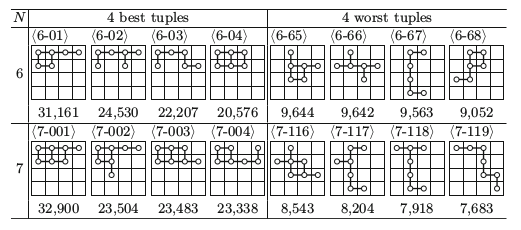
\includegraphics[width=10cm]{figure_004.png}
	\caption{最も優れている/劣っている上位4つの6タプル・7タプル (Oka \& Matsuzaki)}
	\label{figure_004}
	\end{center}
\end{figure}

\subsection{nタプルネットワークに組み込むnタプルの数の検討}
6タプルおよび7タプルの性能が判明したので,性能が良い任意の数のタプルを組み合わせてnタプルネットワークを作成することが可能になった.Szubert \& Ja\'{s}kowskiおよびWuは4個のタプルを組み合わせてnタプルネットワークを作成していたが,Oka \& Matsuzakiは5個以上のタプルを組み合わせることを検討した.すなわち,nタプルの数が多くなればなるほどnタプルネットワーク全体としての性能も上がると思われるが,最も性能が良くなるタプルの数は何個かを明らかにするということである.

実験においては,6タプルの場合最大で上位45個,7タプルの場合最大で上位10個のタプルからnタプルネットワークを作成することとした.各nタプルネットワークに対して,600万ゲーム学習を行わせ,10,000ゲームごとに平均スコアと最大スコアを記録した.その結果が図\ref{figure_005}である.左上のグラフは性能上位$m$個の6タプルによるnタプルネットワークを用いた学習器の成績のうち,平均スコアを示す.右上のグラフは性能上位$m$個の7タプルによる学習器の平均スコアを,左下のグラフは性能上位$m$個の6タプルによる学習器の最高スコアを,右下のグラフは性能上位$m$個の7タプルによる学習器の最高スコアを示す.

\begin{figure}[t]
	\begin{center}
	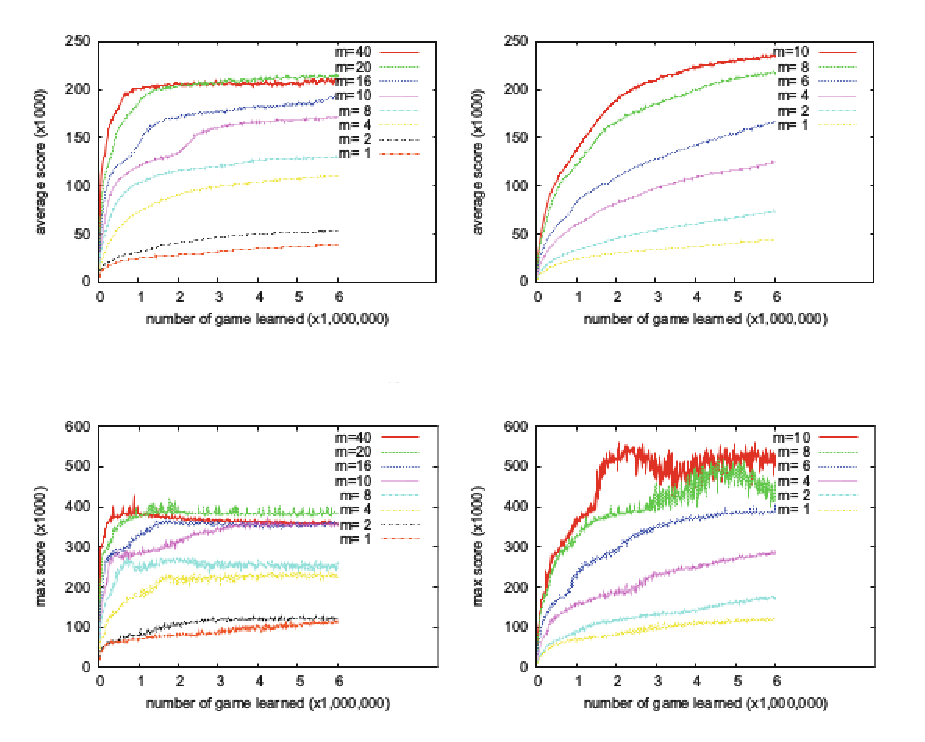
\includegraphics[width=11cm]{figure_005.eps}
	\caption{成績上位タプルm個を組み合わせたタプルネットワークの実験.図の左列は6タプル,右列は7タプルによるネットワークによる実験の結果である (Oka \& Matsuzaki)}
	\label{figure_005}
	\end{center}
\end{figure}

上記の通り,実験群の中では10個の7タプルを組み合わせたタプルネットワークが最も良い成績を収めることがわかった.なお,グラフからも読み取れるが,7タプルによるネットワークに関しては600万ゲーム学習しても平均スコア・最高スコアが収束しない.そのためさらに組み合わせるタプルを増やすとさらに成績が良くなることが考えられるが,技術上の制約により$m=11$以上は実現できなかった\footnote{7タプルを組み合わせてタプルネットワークを作成する場合,重みを保持するために1個のタプルにつき1GBのメモリを消費しなければならない.Oka \& Matsuzakiが実験を行った環境はメモリが12GBしか確保できなかったため,$m=11$以上は実験を行うことが困難だったのではないかと考えられる.また,この研究においてゲーム木探索を組み込むことができなかったのもメモリの制約が原因ではないかと考えられる}.

\subsection{結果と課題}
Oka \& Matsuzakiの研究における最も良いnタプルネットワークは,勝率が0.9850,平均スコアが234,136,最高スコアが504,660という成績を残した.これはゲーム木探索を用いない計算機を用いた2048プレイヤとしては最も良い成績であった.しかしながら,ゲーム木探索を用いなかったことによりゲーム序盤では安定性を欠いてしまい,Wuが達成した勝率1を割り込む形となってしまったし,単純に2048プレイヤとしての成績を比べるとWuのものよりも平均スコア・最大スコアともに低くなっている.一方で,ゲーム木探索を採用しなかったことはプログラムの高速化という点では利があり,1秒あたり88000手の遷移を行うことができるプログラムとなった.これはWuの研究と比べて約290倍高速である.

\section{Yeh et al. (2016)}
YehはWu et al. (2014)の研究にも参画していた共同研究者で,Wuの研究の流れを引き継ぐ形で2048プレイヤの改良を行った.Wuの研究で用いたMS-TD学習の考え方,改良されたnタプルネットワーク,Expectimax木探索は引き続き用いられているため,この研究で新たに加わった要素のみを述べる.

\subsection{新たな特徴量の追加}
Yehは,nタプルネットワークによる学習の他に,盤面に表れる種々の特徴量を追加の価値関数として用いることとした.盤面の評価値には従来のnタプルネットワークによる評価値と新たに採用した特徴量による価値関数の和を用い,これをTD学習で訓練した.なお,採用した特徴は以下のつである.

\begin{enumerate}
\item 大きな数が書かれたタイルの個数
\item 何も書かれていないタイルの個数
\item 異なる数が書かれた(distinct)タイルの個数
\item マージすることができるタイルのペアの組数
\item 書かれているタイルの数が$({\nu}, 2{\nu})$の形になっているタイルのペアの個数
\end{enumerate}

\subsection{MS-TD学習のステージ分けの改良}
WuはMS-TD学習を行うにあたり3ステージに分けて訓練・ゲームプレイを行っていたが,このステージの分け方をさらに細かくした.Yehによってテストされたステージ分けは以下の通りである.なお,$T_{x+y+zk}$という表記は,「盤面に初めて$1000x, 1000y, 1000z$のタイルが同時に現れた時」のことを指す.各タイルの数は百の位で切り捨てられて表現されている.

\begin{itemize}
\item \textbf{戦略1}:$T_{8k}, T_{16k}, T_{16+8k}$を境界として4つにステージを分ける
\item \textbf{戦略2}:$T_{16k}, T_{16+8k}, T_{16+8+4k}$を境界として4つにステージを分ける
\item \textbf{戦略3}:$T_{16k}, T_{16+8k}, T_{16+8+4k}, T_{16+8+4+2k}$を境界として5つにステージを分ける
\item \textbf{戦略4}:$T_{16k}, T_{16+8k}, T_{16+8+4k}, T_{16+8+4+2k}, T_{16+8+4+2+1k}$を境界として6つにステージを分ける
\end{itemize}

まず戦略1をテストした際,$T_{8k}$を境界としてステージを分けることは意味がないことがわかったため,戦略2以降では$T_{16k}$以降のステージ分けのみを考えることとした.戦略2から戦略4をテストした結果,平均スコアでは戦略4が最も優秀であることがわかったが,最高スコアと32678-タイルの到達率では戦略3が最も優秀であった.各戦略ごとの成績は表\ref{tab:yehMultistage}の通りである.各学習器は3手先読みによるゲームプレイを行っており,最高スコアを除く各指標は10,000ゲームの検証ゲームの結果の平均である.

\begin{table}[t]
\newcolumntype{C}{>{\centering}p{5em}}
	\begin{center}
		\caption{戦略1〜4のステージ分けによるMS-TD学習で訓練した学習器の成績 (Yeh et al.)}
		\begin{tabular}{l|C|C|C|C} \hline
		 & 戦略1 & 戦略2 & 戦略3 & 戦略4 \tabularnewline \hline \hline
		16384-タイル作成率 & 87.23\% $(\pm 0.65\%)$ & 87.68\% $(\pm 0.64\%)$ & 87.68\% $(\pm 0.64\%)$ & 87.68\% $(\pm 0.64\%)$ \tabularnewline \hline
		32768-タイル作成率 & 14.15\% $(\pm 0.68\%)$ & 15.30\% $(\pm 0.71\%)$ & 18.31\% $(\pm 0.76\%)$ & 16.82\% $(\pm 0.73\%)$ \tabularnewline \hline
		最高スコア & 594,716 $(\pm 51,886)$ & 579,996 $(\pm 40,583)$ & 614,204 $(\pm 10,053)$ & 610,011 $(\pm 13,720)$ \tabularnewline \hline
		平均スコア & 349,996 $(\pm 3,433)$ & 350,150 $(\pm 9,097)$ & 361,395 $(\pm 9,892)$ & 364,438 $(\pm 9,448)$ \tabularnewline \hline
		速度(手数/秒) & 1,152 $(\pm 93)$ & 1,165 $(\pm 114)$ & 1,106 $(\pm 106)$ & 1,078 $(\pm 104)$ \tabularnewline \hline
		\end{tabular}
		\label{tab:yehMultistage}
	\end{center}
\end{table}

以上の結果より,Yehは戦略3が最も優れたステージ分けだと判断し,これ以降は戦略3を用いて実験を行った.

\subsection{学習率の調整}
TD学習をより正確に行うために,まず学習率$\alpha = 0.0025$でTD学習を行った後,価値関数に大きな改善が見られなくなったと判断したら,学習率$\alpha = 0.00025$に変更して学習を続行させるようにした.

\subsection{TD(${\lambda}$)の使用}
Szubert \& Ja\'{s}kowskiおよびWuはTD学習においてTD(0)を使用していたが,将来の盤面と報酬を見通しながら学習を行うために,YehはTD(${\lambda}$)の導入を行った.Yehは${\lambda}=0.5$とし,前方の5ステップ・バックアップの報酬を平均化することとした.目標とする収益$R^{\lambda}_t$は以下の式の通りである.

\[
R^{\lambda}_t = 0.5R^1_t + 0.25R^2_t + 0.125R^3_t + 0.0625R^4_t + 0.0625R^5_t
\]

なお,$R^n_t$は$R^n_t = \sum_{k=0}^{n-1} + V(s_{t+n})$で与えられる.

\subsection{結果}
上記の改良を重ねた結果,Yehは平均スコア443,526,最大スコア793,835と非常に良い成績の学習器を訓練することに成功した.なお,32678-タイルへの到達率は31.75\%,1秒あたりの遷移速度は500手であった.さらに,検証ゲーム中のある1ゲームにおいて65536-タイルを生成することにも成功した.これは強化学習ベースの2048プレイヤでは当時として最も強く,Xiaoのよる深い先読みによる探索ベースのものよりも平均スコアでは優っており,Yehの方が125倍速いプログラムであった.

\section{Ja\'{s}kowski (2017)}
Ja\'{s}kowskiは,Yehまでの2048プレイヤの改良の流れを受け継ぎながら,これまで用いられてきたTD学習や訓練・検証のステージ分けなどに対して改良を加えつつ,新たな手法を加えることでさらに優秀なプレイヤの実装を目指した.

\subsection{自動的な学習率決定アルゴリズムの適用}
Ja\'{s}kowskiはTD(${\lambda}$)を使用する点はYehの研究を継承したが,TD学習で最も重要なパラメータである学習率を決定するにあたり,新たな手法を提案した.すなわち,Yehの研究では手動で学習率が設定されていたのに対して,Ja\'{s}kowskiはこれまでに提案されてきたオンライン適応学習による学習率決定のアルゴリズムを2048にも適用することを試みた.

Bagheri et al.によるConnect 4\footnote{いわゆる「四目並べ」に近い2プレイヤ対戦型のボードゲーム}への適用の研究において,これらの学習率決定アルゴリズムはいずれも標準的なTD学習よりも良い成績を残すことが明らかとなったが\cite{Bagheri},一方で長期的に見るとアルゴリズム間の差はそこまで大きいものにはならなかった.そこで,Ja\'{s}kowskiは最もシンプルなTemporal Coherence(TC(${\lambda}$))と,より先進的でチューニングの必要がないAutostepを選択して実験することにした.

\subsubsection{TC(${\lambda}$)}
これまでのTD(${\lambda}$)では実験者が学習率${\alpha}$を手動で決定していたが,TC(${\lambda}$)においては,手動で決定される${\alpha}$の代わりに以下のパラメータを用いて学習率${\gamma}$を決定する.

\begin{itemize}
\item \textbf{メタ学習率${\beta}$}:実験者が手動で設定するパラメータ
\item \textbf{累積誤差関数$E(s)$}:これまでTD学習で価値関数$V(s)$の更新を行う際に用いてきた誤差${\delta}_t = r_{t+1} + V(s_{t+1}) - V(s_t)$を,$V(s)$の更新を行う際に$E(s)$に対して加算する.盤面$s$は価値関数と同様に,nタプルネットワークを用いて近似される
\item \textbf{累積絶対誤差関数$A(s)$}:$V(s)$の更新を行う際に,${\delta}_t$の絶対値を$A(s)$に対して加算する.盤面$s$は価値関数と同様に,nタプルネットワークを用いて近似される
\item \textbf{適応学習率${\alpha}$}:$E(s)$と$A(s)$の値によって自動的に決定されるパラメータ
\end{itemize}

適応学習率${\alpha}$は以下の式で求められる.

\[
{\alpha} = 
\begin{cases}
\dfrac{|E_i[s'_k]|}{A_i[s'_k]}, & \text{if $A_i[s'_k] \neq 0$} \\
1 & \text{otherwise}
\end{cases}
\]

また,学習率${\gamma}$は以下の式で求められる.

\[
{\gamma} = \dfrac{{\alpha} \times {\beta}}{m} \;\; \text{($m$はnタプルネットワークに格納されているタプルの数)}
\]

このような学習率の求め方をすることによって,累積誤差と累積絶対誤差の値が近い場合は学習率が大きく,逆に累積誤差と累積絶対誤差の差が大きくなると学習率は小さくなる.ある盤面$s$に対して累積誤差$E(s)$と累積絶対誤差$A(s)$の差が大きいということは,$s$に対して負の値の${\delta}_t$が加算されることが多くなっているということであり,すなわちそれはこの盤面に対しての価値関数の評価が上手く行っていないということであるから,学習率を低くして価値関数の更新を穏やかに行うのは理にかなっていると考えられる.

\subsubsection{Autostep}
AutostepはMahmood\cite{Mahmood}によって提案されたアルゴリズムで,SuttonによるIDBD\cite{IDBD}の拡張にあたる.Autostepでは,ステップサイズの上限を定め,もしステップサイズが大きくなりすぎていることが検知されたらステップサイズ値を小さくするという方法で,IDBDを改良したものである.Autostepでは3種類のパラメータを設定する必要があり,Ja\'{s}kowskiの研究では,このうち初期ステップサイズ${\alpha}_{init} = 1.0$,割引率${\tau} = 0.0001$は固定され,メタ学習率${\mu}$の値をいくつか選択して実験が行われた.

\subsubsection{結果}
Ja\'{s}kowskiは,前述の2つの自動的な学習率決定アルゴリズムに加え,従来のTD学習\footnote{TC(${\lambda}$)およびTD(${\lambda}$)においては,${\lambda}=0.5$とした}を採用した合計3種類の手法で,1手先読み(すなわち,先読みを行わない)と3手先読みの2つの条件で実験を行った.その結果,全ての学習率決定手法のうち,1手先読みの場合はTC(${\lambda}$)で${\beta}=1.0$の時に平均スコアが最も良くなり,3手先読みの場合はTC(${\lambda}$)で${\beta}=0.5$の時に平均スコアが最も良くなった.1手先読み・3手先読みの場合ともに,TD(${\lambda}$)およびAutostepはどのように学習率・メタ学習率を設定してもTC(${\lambda}$)に優る平均スコアを達成することはできなかった.

Ja\'{s}kowskiは,Autostepは定常的な教師データが存在する作業に特化しているため,訓練データが定常的ではない2048にはあまり適していなかったと考えている.また,TC(${\lambda}$)およびAutostep両者に共通する欠点として,何かしらの近似した盤面に対応する重みを保持する必要があることから,TD(${\lambda}$)よりも多くのnタプルネットワークを保持しなければならないため,計算時間が長くなってしまうことを指摘している.

\subsection{Multi-Stage Weight Promotion}
Ja\'{s}kowskiはWuが提案したMS-TD学習の考え方を概ね継承したが,ステージ分けと重みの選択において細かい改良を加えた.

\subsubsection{新しいステージ分け}
Wuでは3ステージ,Yehでは5ステージに分けることが最善であるとされていたステージ分けについて,Ja\'{s}kowskiは$2^g$ステージに分け($g$は正の整数),また各ステージの「長さ」$l$を$l = 2^{15+1-g}$と定義した.例えば$g=4$の時,長さ$l=2^{12}=4096$である.この場合,以下のようなステージ分けがなされる.

\begin{enumerate}
\item ステージ1:初期盤面から$T_{4096}$まで
\item ステージ2:$T_{4096}$から$T_{8192}$まで
\item ステージ3:$T_{8192}$から$T_{8192+4096}$まで
\item ステージ4:$T_{8192+4096}$から$T_{16384}$まで
\item ...
\item ステージ16:$T_{32768+16384+8192+4096}$から$T_{65536}$まで
\end{enumerate}

なお,TC(${\lambda}$)で導入した累積誤差関数$E$と累積絶対誤差関数$A$についても同様にステージ分けを行って重みを保持する.

\subsubsection{Weight Promotion}
WuおよびYehのステージ分けにおいては,新しいステージの学習を始める際に再び何も学習していない状態からnタプルネットワークの訓練を行わなければならなかったため,汎化性能が著しく損なわれていた.この汎化性能の弱体化はステージ数が多くなればなるほど進むため,Yehはステージを多くすれば多くするほど学習器の性能は悪くなることを指摘しており,その結果5ステージに分けるのが最も良いと考えたのである.この問題を「ステージ数を多くしない」以外の方法で解決するために,Ja\'{s}kowskiは各ステージの初期状態の評価値を,前のステージの同じ盤面から引き継ぐことにした.Ja\'{s}kowskiはこの方策をWeight Promotionと呼び,上記の多段ステージ分けとともに提案した.

\subsubsection{結果}
Ja\'{s}kowskiは,以下の6つの条件について,1手先読みと3手先読みの2つの条件を掛けあわせて合計12の実験を行った.なお,WPはWeight Promotionを適用したことを示し,6. 以外の5つの実験においては全て共通の5つの6タプルによる実験を行った.

\begin{enumerate}
\item ステージ分けを行わない(純然たるTC(${\lambda}$))
\item $g=4$
\item $g=3, WP$
\item $g=4, WP$
\item $g=5, WP$
\item 5つの7タプルによるTC(${\lambda}$)で,ステージ分けを行わない
\end{enumerate}

この結果,1手先読みでは6. の7タプルによるTC(${\lambda}$)が最も良い成績を収め,1. に関しても2. と5. の実験には成績が優るなど,ステージ分けに対しては顕著な効果が見られなかった.一方3手先読みでは4. の実験が最も良い成績を収め,ステージ分けを行わない1. と6. の実験よりも高い平均スコアを得た.また学習プロセスに注目すると,ステージ分けを行う実験では平均スコアが単調増加していたのに対し,ステージ分けを行わない場合は平均スコアが逆に悪くなっていることが確認された.

以上の結果より,Ja\'{s}kowskiはステージ分けを行わない学習器は1手先読みの条件に対して過学習が起きてしまうが,ステージ分けを行う学習器は過学習に耐性があり,成績の悪化は起こらなくなると結論付けた.なお,Weight Promotionについては1手先読みに対しても3手先読みに対しても適用することでより良い成績が得られることが確認された.

\subsection{Carousel Shapingと余剰タプルの追加}
\subsubsection{Carousel Shaping}
前節のステージ分けにおける改良を行った際,従来の学習器は1手先読みの条件の下で過学習を行ってしまい,3手先読みでは学習を重ねるに従って成績を落としてしまうという状況が確認された.これは従来のMulti-Stage学習ではゲームで重要になる終盤のステージでの学習時間が少なくなってしまうことが原因であると考えたJa\'{s}kowskiは,終盤のステージにおける学習時間を確保するため,Carousel Shapingという新たなMulti-Stage学習の手法を提案した.Carousel Shapingの擬似コードをAlgorithm \ref{alg1}に示す.

\begin{algorithm}
\caption{Carousel Shaping}
\label{alg1}
\begin{algorithmic}[1]
\STATE \textbf{function} \textsc{CarouselShaping}
\STATE  $stage \leftarrow 1$
\STATE  $initstates[x] = \emptyset$ \textbf{for} $x \in \{1...2^g\}$
\STATE  \textbf{while not} enough learning \textbf{do}
\STATE   \textbf{if} $stage = 1$ \textbf{then}
\STATE    $s \leftarrow$ \textsc{InitialState()}
\STATE   \textbf{else}
\STATE    $s \leftarrow$ \textsc{RandomChoice}$(initstates[stage])$
\STATE   \textsc{LearnFromEpisode}$(s)$ $\triangleright$ Updates $initstates$
\STATE   $stage \leftarrow stage + 1$
\STATE   \textbf{if} $stage > 2^g$ \textbf{or} $initstates[stage] = \emptyset$ \textbf{then}
\STATE    $stage \leftarrow 1$
\STATE \textbf{end function}
\end{algorithmic}
\end{algorithm}

Carousel Shaping(CS)では,明確に学習を行うステージを分けるのではなく,1回のゲームの中で複数のステージにまたがった学習を可能にする.ステージ1の初期盤面から学習を始め,もし途中でステージ分けの境界にあたる盤面に到達したならその都度$initstates$に登録しつつ\footnote{\textit{initstates}は各ステージの初期盤面を保持するデータ構造で,各ステージごとに最近到達された初期盤面1000個を保持する}学習を行う.学習が1ゲーム分終わったら次のステージに進み,そのステージの初期盤面を取得し,学習を行う.もしステージが$2^g$を超えるか,そのステージの初期盤面がまだ1つも記録されていなかった場合,ステージ1に戻って学習を行う.このように,CSはその名(carousel=回転木馬)の通り学習するステージをローテーションさせながら学習を行う.

\subsubsection{余剰タプルの追加}
Ja\'{s}kowskiが導入した最後の手法が余剰タプルの追加(Redundant Encoding)である.これまで使用してきた5個の6タプルに加え,より小さい2個の3タプルと5個の4タプルをタプルネットワークに加えて学習を行う.ここで追加したタプルは既に使用しているタプルの形状の中に含まれているため,一見すると無意味なタプルではあるが,追加することでより速く汎化することが確認された.ただし,サイズが小さいとはいえ7個のタプルを追加するため,学習時間は非常に長くなる.

\subsection{結果}
以上の改良を加え,さらにExpectimax木探索による探索を,先読みする手数ではなく1手あたり1000ミリ秒という時間単位で許容したところ,Ja\'{s}kowskiによる2048プレイヤは平均スコア609,104を記録した.これは先行研究のいずれよりも優れた成績である.またこの研究における最も優秀なプレイヤは1秒に1手のペースでアクションを選択するため,1秒あたり500手進めることができるYehのものより表面上は遅くなるが,仮に1秒に上限1000手のペースでアクションを選択するよう調整した場合は平均スコアが527,099となり,Yehの443,526を上回る.すなわち,学習のみならず検証時のプレイにおいてもYehのプレイヤよりも性能が高いということになる.

\chapter{ヒューリスティックス}
先行研究で挙げられてきた2048プレイヤは,強化学習によって有り得る2048の盤面の評価値を記録しておき,盤面に応じて最も価値が高いと思われる盤面につながるアクションを選択するという方策のもとにプレイを行ってきた.翻って人間が2048をプレイする場合,人間が盤面の価値を評価・記憶することは明らかに不可能である.そのため,人間が2048をプレイする際には,ある一定の方策をいくつか持ち,その方策に従う盤面を導き出すようにアクションを選択していると考えられる.ここで,人間が採用していると考えられる2048の方策をいくつか挙げる.

\section{base方策}
人間が2048をプレイする時,一般的に大きな数のタイルを盤面のうちいずれか1辺に寄せようとする傾向がある.この方策を\textbf{base方策}と名付けることとする.base方策に基づいたプレイのフローの例は以下の通りである.

\begin{itemize}
\item 盤面の任意の辺4マスに「基地」(base)を作って,大きなタイルを蓄える場所と決めておく\footnote{プレイヤ自身の好みによって下や左などの辺が基地に選ばれるが,どの辺を選んだとしても対称な盤面を作ることができるので,どの辺を基地に選んでも実質的に変わらないと考えられる}
\item 基地以外の残りの9マスを使って,新しく数の大きいタイルを作成する
\item 基地にマージできるタイルを作成できたら,基地にあるタイルへマージする
\item 基地内でマージすることができるタイルの組ができたら,それらをマージし,さらに大きな数のタイルにする
\end{itemize}

もし基地を定めない場合,大きなタイルが盤面のあちらこちらへ移動することとなる.$2{\nu}$-タイルを作成することが困難な${\nu}$-タイル──例えば2048-タイルなどが盤面を上下左右に移動することを考えると,例えば4-タイルや8-タイルといった小さなタイルのマージを行う妨げとなり,盤面の自由度が極端に下がる.そのため,より長くゲームを行うためにはbase方策に従うことが重要であると考えられる.

\section{array方策}
人間がbase方策に従って2048プレイする際,基地の中ではできる限りタイルが「$2^{k}-2^{l}-2^{m}-2^{n} \;\; (0<k<l<m<n)$」といった形へ,タイルの数が降順もしくは昇順になるように整列(array)させる傾向がある.この方策を\textbf{array方策}と名付けることとする.

この方策はbase方策との相乗効果が高い.例えば「$32-64-128-256$」という順列の基地を作った場合,基地の外で32-タイルの作成に成功すれば,そのまま基地内でマージを行うことによって512-タイルを作成することができる.あるいは,基地の外で128-タイルの作成に成功した場合はマージを行うと「$32-64-512$」となるが,この状態でもarray方策は維持されており,ゲームを長く進めていても保持しやすい性質である.

\section{maximum-in-corner方策}
最後に,最もシンプルな方策として\textbf{maximum-in-corner方策}を挙げる.この方策では,現状の盤面における$max tile$が四隅のどれかのマスにあることを重視する.これはarray方策の拡張的な方策と考えられる.例えば「$2-32-2048-2$」という順列の基地を考えると,前の3つのタイルはarray方策に従っているものの,「$2048-2$」という並びはarray方策に反している.この状況を解決するためには,以下のいずれかの操作が必要になる.

\begin{enumerate}
\item 2および32にタイルをマージし続け,2048-タイルを作成し,既に存在している2048-タイルとマージする
\item 2048に隣接している2-タイルを基地の外へと移動させ,2048-タイルを順列の終端へと移動させる
\end{enumerate}

このうち,1. を実現させることは難しいと考えられる.なぜなら,基地のうち2マスがマージすることができないタイルで占められているため,より少ないバッファでタイルをマージすることが必要になるからである.一方で,2. を実現させることも同様に難しい.横もしくは縦一列に並んでいるタイルの中から,1つだけを選んで基地から外す操作をすることを,意図して行うのは難しい.したがって,一度array方策に反する順列を作ってしまった場合,array方策に従うような順列に復帰させることは非常に難しいということになる.

このような困難な状況に陥ることを防ぐため,あらかじめarray方策に反する順列を作らないような方策が必要になる.これがmaximum-in-corner方策であり,大きな数のタイルができる限り盤面の隅から離れないことで,よりarray方策を長く実現できるようにしている.

\section{ヒューリスティックスと強化学習によるプレイヤの関係}
強化学習によって訓練された2048プレイヤがこれらの方策に従っているかどうかを確かめるために,各方策に2048の盤面がどれぐらい従っているかを定量的に表現する評価関数を実装した.それぞれの評価関数の定義は以下の通りである.これらの3つのスコアを1ゲーム中全ての盤面に対して算出し,その総和を盤面の数で割った値をそのゲームの各スコアの代表値とする.

\begin{itemize}
\item \textbf{base方策:}盤面上で最も大きな数のタイルのうち,上位4個のタイルの数の和を${\sigma}$とする.盤面の終端にある4辺のうち,最も大きな数のタイルが集まっている辺を選び,その辺のタイルの数の和を${\pi}$とする.$\displaystyle \frac{\sigma}{\pi}$をこの盤面の\textbf{base方策スコア}とする
\item \textbf{array方策:}盤面上のbaseにおけるタイルの並びにより,以下の通り\textbf{array方策スコア}を決定する:
\begin{itemize}
\item baseの左端から右端まで一度も順列の昇順/降順が逆転しなかった場合,2点とする
\item baseの左端から右端までの間,1回だけ順列の昇順/降順が逆転した場合,1点とする
\item baseの左端から右端までの間,2回順列の昇順/降順が逆転した場合,0点とする
\end{itemize}
\item \textbf{maximum-in-corner方策:}盤面の四隅のうちいずれかのマスに$maxtile$が存在するなら,\textbf{maximum-in-corner方策スコア}を1点とする.この条件を満たさないならmaximum-in-corner方策スコアは0点である
\end{itemize}

これらのスコアが強化学習によって訓練されたプレイヤにおいて習得されていることを示すため,ランダムプレイヤ\footnote{全ての盤面において可能なアクションの中からランダムにアクションを選択するプレイヤ}において1000ゲームを行った際のスコアと,強化学習により価値関数の訓練を500,000ゲームにわたって行ったプレイヤにおいて1,000ゲームの検証ゲームを行った際のスコアを比較した.その結果,全ての方策スコアについて,99\%以上有意に強化学習によるプレイヤの方が優れていることを示した.以上により,強化学習により価値関数の訓練を行ったプレイヤは,各方策を自然と習得していることが示された.

ところで,強化学習によるプレイヤのbase方策スコアの平均値は0.912であった.この値が1であれば全ての盤面においてbase方策が守られていることになるが,ゲーム終盤においてタイルの移動が制限されるとbase方策を守ることが難しくなることを考慮すると,base方策はかなり高い確率で守られると考えられる.一方でarray方策スコアの平均値は1.61,maximum-in-corner方策スコアの平均値は0.816であった.base方策が“満点”の9割を達成していたことを考えると,これらのスコアはやや低めである.また前述の通りmaximum-in-corner方策はarray方策の拡張的な方策であるから,maximum-in-corner方策スコアが改善すればarray方策スコアも改善する可能性があり,その結果プレイヤの性能が向上すると考えられる.

以上より,本研究においては特にmaximum-in-corner方策に注目し,先行研究の強化学習を使用したプレイヤに対してより強くmaximum-in-corner方策に従うような改修を導入することによって,2048プレイヤの性能に一定の改善が見られるものと考えた.

\chapter{提案と実装}
\section{maximum-in-corner方策の導入}
強化学習を用いて盤面ごとに評価値を学習した2048プレイヤにおいてmaximum-in-corner方策を導入する場合,強化学習によって訓練された価値関数$V(s)$を\emph{ある程度}尊重しつつ,maximum-in-corner方策に従ってアクションの選択がなされるように,方策に従っている評価値を割り増して評価する必要がある.そのため本研究においては,以下のようにmaximum-in-corner方策を適用することとした.

\begin{enumerate}
\item アクション選択の手順において,選択可能なアクションを$a_n \;\; (0 \leq n < 4)$とする.
\item 選択可能なアクションを元に,遷移を行った後の盤面$s_{a_n}$を求める.
\item 求められた盤面に対する評価値$V(s_{a_n})$を求める.
\begin{itemize}
\item この時,もし$s_{a_n}$の$maxtile$が盤面の四隅のいずれかのマスにあるならば,$V(s_{a_n}) = {\rho} \times V(s_{a_n})$とする.${\rho}$は実験者が設定する$1$以上の定数であり,この定数のことを\textbf{corner ratio}と呼ぶこととする.
\end{itemize}
\item 評価値を全ての有り得る盤面に対して求めた後,最も大きな$V(s_{a_n})$を与えるアクション$a_n$を選択する.
\end{enumerate}

この実装によって,「価値関数$V(s)$を\emph{ある程度}尊重しつつ方策に従っている評価値を割り増して評価する」というプレイヤの挙動を,以下のように表現することが可能になる.ここで,maximum-in-corner方策に従うアクションの中で(corner ratioによる割増前に)最も大きな評価値を与えるアクションを$a_{\sigma}$,maximum-in-corner方策に従わないアクションの中で最も大きな評価値を与えるアクションを$a_{\tau}$とする.

\subsection{$V(s_{a_{\sigma}}) > V(s_{a_{\tau}})$の場合}
corner ratioによる割増を行わなくても,$a_{\sigma}$が選択できるアクションの中で最も大きな評価値を与えるアクションであるから,$a_{\sigma}$が選択される.このアクション選択は強化学習による価値関数とmaximum-in-corner方策の両方に従っている.

\subsection{$V(s_{a_{\sigma}}) < V(s_{a_{\tau}})$かつ${\rho}V(s_{a_{\sigma}}) > V(s_{a_{\tau}})$の場合}
corner ratioによる割増を行わなければ,$a_{\tau}$が選択できるアクションの中で最も大きな評価値を与えるアクションである.しかしながら,評価値の割増を行うと${\rho}V(s_{a_{\sigma}})$の方が大きな評価値を与えるから,結果としては$a_{\sigma}$が選択される.この場合,$V(s_{a_{\sigma}})$と$V(s_{a_{\tau}})$の差は小さいため,僅かに評価値が高いもののmaximum-in-corner方策には従わないアクションを選択するのであれば,僅かに評価値が低いがmaximum-in-corner方策に従うアクションを選択したほうが良いという考えに基づき,割増込みで高い評価値を与えるアクション$a_{\sigma}$が選択される.

\subsection{$V(s_{a_{\sigma}}) < V(s_{a_{\tau}})$かつ${\rho}V(s_{a_{\sigma}}) < V(s_{a_{\tau}})$の場合}
corner ratioによる割増を行わない場合は$a_{\tau}$が最も大きな評価値を与えるアクションであるが,割増を行ったとしても$a_{\tau}$が最も大きな評価値を与えるということは変わらない.この場合,学習によって$a_{\tau}$がmaximum-in-corner方策に従うアクションと比べて非常に良いアクションであると判断されたということになるので,maximum-in-corner方策はここでは棄却し,強化学習によって導かれた最善のアクションを選択する.

\bigskip

なお,上記の場合分けにおいては$V(s_{a_{\sigma}}) < V(s_{a_{\tau}})$かつ${\rho}V(s_{a_{\sigma}}) < V(s_{a_{\tau}})$の場合のみmaximum-in-corner方策を棄却したが,実際は$V(s_{a_{\sigma}}) < V(s_{a_{\tau}})$かつ${\rho}V(s_{a_{\sigma}}) > V(s_{a_{\tau}})$の場合においてもmaximum-in-corner方策を棄却した方が良かったという場合が存在する可能性がある.このような,「誤ってmaximum-in-corner方策に従ってしまったが,実際は従わなかった方が良かった」という状況のことを,\textbf{corner誤謬}と呼ぶことにする.基本的に本研究においては,たとえcorner誤謬が存在していたとしてもmaximum-in-corner方策を導入することにより得られる効用の方が大きいと考えるが,corner誤謬による弊害が大きくなった場合,すなわちmaximum-in-corner方策を使用しないプレイヤと比べて使用するプレイヤの性能が悪くなってしまう場合は,maximum-in-corner方策の導入の方法について検討し直す必要があることに留意しておく.

\section{実装}
まず,maximum-in-corner方策を採用せず,遷移後盤面を評価する通常のTD学習の擬似コードをAlgorithm \ref{alg2}に示す.この擬似コードはSzubert \& Ja\'{s}kowskiの実装に基づく.なお,\textsc{ValidActions}$(s)$は盤面$s$に対して選択可能なアクションの集合を返す関数,\textsc{ComputeAfterstate}$(s,a)$は盤面$s$とアクション$a$に対して遷移後の盤面$s'$と報酬$r$を返す関数,\textsc{InitializeGameState()}は初期盤面を返す関数,\textsc{IsTerminalState}$(s)$は盤面$s$が終末盤面ならばtrueを返す関数,\textsc{GetNextState}$(s)$は遷移後の盤面$s$に対してランダムタイルを生成する関数である.

本研究においては,Algorithm\ref{alg2}のうち,関数\textsc{ChooseBestTransitionAfterstate}にAlgorithm\ref{alg3}の9行目から11行目を加えた関数\textsc{ChooseBestTransitionAfterstateCorner}を実装すると同時に,その盤面の$maxtile$が四隅のマスにあるかどうかを判断する関数\textsc{IsMaxtileInCorner}を実装する.

なお,\textsc{ChooseBestTransitionAfterstate}は,nタプルネットワークを用いてプレイする\footnote{ここでの「プレイ」とは,検証ゲームを行うという意味である}関数\textsc{PlayGame}およびnタプルネットワークを訓練する関数\textsc{LearnEvaluation}に呼ばれている,nタプルネットワークを参照して最も良い遷移後盤面と報酬を返す関数である.\textsc{ChooseBestTransitionAfterstate}と\textsc{ChooseBestTransitionAfterstateCorner}を両方実装しておいて,検証ゲームを行う際にどちらかの関数を呼ぶようにすることで,検証ゲームと学習ゲームのどちらか,もしくはそのどちらもにおいてmaximum-in-corner方策を採用することができるようになる.

\medskip

\begin{breakablealgorithm}
\caption{Temporal Difference Learning (TD(0))}
\label{alg2}
\begin{algorithmic}[1]
\STATE \textbf{function} \textsc{GetBestValueAction}$(s)$
\STATE  $A(s) \leftarrow $ \textsc{ValidActions}$(s)$
\STATE  $bestValue \leftarrow -\infty$
\STATE  \textbf{for all} $a$ \textbf{such that} $a \in A(s)$ \textbf{do}
\STATE   $s', r \leftarrow$ \textsc{ComputeAfterstate}$(s,a)$
\STATE   $value \leftarrow r + V(s')$
\STATE   \textbf{if} $(value > bestValue)$ \textbf{then}
\STATE    $bestValue \leftarrow value$
\STATE   \textbf{endif}
\STATE  \textbf{endfor}
\STATE  \textbf{return} $bestValue$
\STATE \textbf{end function}
\STATE
\STATE \textbf{function} \textsc{ChooseBestTransitionAfterstate}$(s)$
\STATE  $A(s) \leftarrow$ \textsc{ValidActions}$(s)$
\STATE  $bestValue \leftarrow -\infty$
\STATE  $bestAfterstate$ 
\STATE  $bestReward \leftarrow 0$
\STATE  \textbf{for all} $a$ \textbf{such that} $a \in A(s)$ \textbf{do}
\STATE   $s', r \leftarrow$ \textsc{ComputeAfterstate}$(s,a)$
\STATE   $value \leftarrow r + V(s')$
\STATE   \textbf{if} $(value > bestValue)$ \textbf{then}
\STATE    $bestValue \leftarrow value$
\STATE    $bestAfterstate \leftarrow s'$
\STATE    $bestReward \leftarrow r$
\STATE   \textbf{endif}
\STATE  \textbf{endfor}
\STATE  \textbf{return} $bestAfterstate, bestReward$
\STATE \textbf{end function}
\STATE
\STATE \textbf{function} \textsc{PlayGame}
\STATE  $score \leftarrow 0$
\STATE  $state \leftarrow$ \textsc{InitializeGameState()}
\STATE  \textbf{while } $\neg$\textsc{IsTerminalState}$(s)$ \textbf{do}
\STATE   $s', r \leftarrow$ \textsc{ChooseBestTransitionAfterstate}$(s)$
\STATE   $s'' \leftarrow $ \textsc{GetNextState}$(s')$
\STATE   $score \leftarrow score + r$
\STATE   $s \leftarrow s''$
\STATE  \textbf{endwhile}
\STATE  \textbf{return} $score$
\STATE \textbf{end function}
\STATE
\STATE \textbf{function} \textsc{LearnEvaluation}
\STATE  $score \leftarrow 0$
\STATE  $targetValue \leftarrow 0$
\STATE  $state \leftarrow$ \textsc{InitializeGameState()}
\STATE  \textbf{while } $\neg$\textsc{IsTerminalState}$(s)$ \textbf{do}
\STATE   $s', r \leftarrow$ \textsc{ChooseBestTransitionAfterstate}$(s)$
\STATE   $s'' \leftarrow $ \textsc{GetNextState}$(s')$
\STATE   $score \leftarrow score + r$
\STATE   $targetValue \leftarrow $ \textsc{GetBestValueAction}$(s'')$
\STATE   $V(s') \leftarrow V(s') + {\alpha}(targetValue - V(s'))$
\STATE   $s \leftarrow s''$
\STATE  \textbf{endwhile}
\STATE \textbf{end function}
\end{algorithmic}
\end{breakablealgorithm}



\begin{algorithm}[t]
\caption{Maximum-in-corner Policy}
\label{alg3}
\begin{algorithmic}[1]
\STATE \textbf{function} \textsc{ChooseBestTransitionAfterstateCorner}$(s)$
\STATE  $A(s) \leftarrow$ \textsc{ValidActions}$(s)$
\STATE  $bestValue \leftarrow -\infty$
\STATE  $bestAfterstate$ 
\STATE  $bestReward \leftarrow 0$
\STATE  \textbf{for all} $a$ \textbf{such that} $a \in A(s)$ \textbf{do}
\STATE   $s', r \leftarrow$ \textsc{ComputeAfterstate}$(s,a)$
\STATE   $value \leftarrow r + V(s')$
\STATE   \textbf{if} \textsc{IsMaxTileCorner}$(s)$ \textbf{then}
\STATE    $value \leftarrow {\rho} \times value$
\STATE   \textbf{endif}
\STATE   \textbf{if} $(value > bestValue)$ \textbf{then}
\STATE    $bestValue \leftarrow value$
\STATE    $bestAfterstate \leftarrow s'$
\STATE    $bestReward \leftarrow r$
\STATE   \textbf{endif}
\STATE  \textbf{endfor}
\STATE  \textbf{return} $bestAfterstate, bestReward$
\STATE \textbf{end function}
\end{algorithmic}
\end{algorithm}



\chapter{実験}
\section{実験1:常に${\rho}=1.2$とする}
まず最初に,maximum-in-corner方策を使用することに効果があるのか調べるため,${\rho}=1.2$として実験を行った.詳細な実験のセッティングは以下の通りである.

\begin{itemize}
\item 学習ゲーム数:500,000
\item 学習率:0.01
\item nタプルネットワークの配置:Szubert \& Ja\'{s}kowskiのスタイル
\item \textsc{ChooseBestTransitionAfterstateCorner}を使用するゲーム:
\begin{itemize}
\item 使用しない(ベースライン)
\item 検証ゲーム
\end{itemize}
\item 使用するcorner ratio:${\rho}=1.2$
\end{itemize}

上記の実験の結果のうち,各検証ゲームにおける平均スコアをグラフにプロットしたのが図\ref{figure_006}である.全体的な傾向としては,約200,000ゲームほどの学習を終えるまでの間はcorner ratioあり,すなわちmaximum-in-corner方策を採用したほうが成績が良い.しかしながら,その後はmaximum-in-corner方策なしの方が全体的に成績が良くなり,一応平均スコアは伸び続けているもののmaximum-in-corner方策ありの方は成績が低調になる.

\begin{figure}[t]
	\begin{center}
	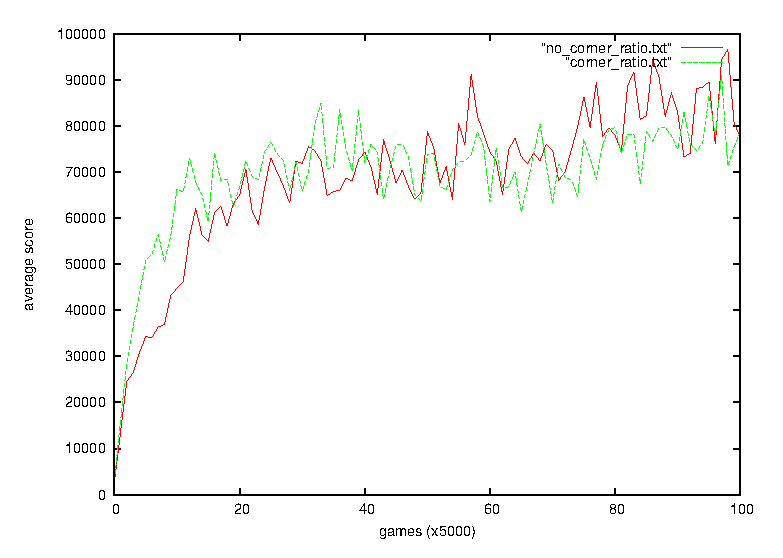
\includegraphics[width=13cm]{figure_006.eps}
	\caption{実験1の結果}
	\label{figure_006}
	\end{center}
\end{figure}

実験1の結果より,高い値のcorner ratioを設定することは学習の序盤において効果があることがわかったが,一方で学習が進むと,かえって学習器の性能を弱めてしまうということがわかった.これらの事実に基づき,以下の仮説を立てた.

\begin{itemize}
\item 一般に,maximum-in-corner方策を採用すること自体は2048プレイヤの性能を高める可能性がある
\item 学習ゲームを重ねるにつれTD学習による学習器の性能は良くなるので,高いcorner ratioの値はcorner誤謬を引き起こす
\end{itemize}

この仮説が正しいことを示すために,corner ratioの適用について様々な条件を用意する追加実験を行うことにした.

\section{実験2:2つの${\rho}$の値を用いる}
実験1においては検証ゲーム中に一貫して${\rho}=1.2$としていたが,学習ゲームが進んだ後にもこの値を使い続けることはあまり良くないということがわかった.そこで,実験2においては,ゲームの状況に応じて異なるcorner ratioの値を使用することとした.また,実験1では検証中のみにmaximum-in-corner方策を採用していたが,実験2においては学習中および検証中と学習中の両方に採用する条件も設定することとした.

なお,ゲームの進行状況を示す指標としては,スコアと$maxtile$を用いることができる.今回の実験ではcorner ratioを変更する指標として,スコアを参照する実験と$maxtile$を参照する実験の両方をそれぞれ行った.詳細な実験のセッティングは以下の通りである.

\begin{itemize}
\item 学習ゲーム数:500,000
\item 学習率:0.01
\item nタプルネットワークの配置:Wuのスタイル\footnote{どのようなnタプルネットワークに対してもmaximum-in-corner方策が適合することを示すために,Szubert \& Ja\'{s}kowskiの実装よりも高級なWuの実装によるnタプルネットワークを用いた}
\item \textsc{ChooseBestTransitionAfterstateCorner}を使用するゲーム:
\begin{itemize}
\item 使用しない(ベースライン)
\item 検証ゲーム
\item 学習ゲーム
\item 検証ゲームと学習ゲームの両方
\end{itemize}
\item 使用するcorner ratio:${\rho}=1.1 \text{もしくは} 1.2$
\item corner ratioを変更する条件:
\begin{itemize}
\item 最初は${\rho}=1.2$とし,スコアが70,000に到達したら${\rho}=1.1$とする
\item 最初は${\rho}=1.2$とし,$maxtile=4096$が達成されたら${\rho}=1.1$とする
\end{itemize}
\end{itemize}

この実験の結果のうち,平均スコアの推移をプロットしたグラフを図\ref{figure_007}から図\ref{figure_009}に示す.実験結果のうち,maximum-in-corner方策を適用しているものについてはいずれもベースラインよりも平均スコアを上回っているが,検証ゲームに適用したものと検証ゲーム・学習ゲームの両方に適用したものについては,顕著にベースラインよりも平均スコアが高くなっている.また全体的な傾向としては,corner ratioを平均する条件にスコアを使用する方が平均スコアが良くなることが多い.

\begin{figure}[tb]
	\begin{center}
	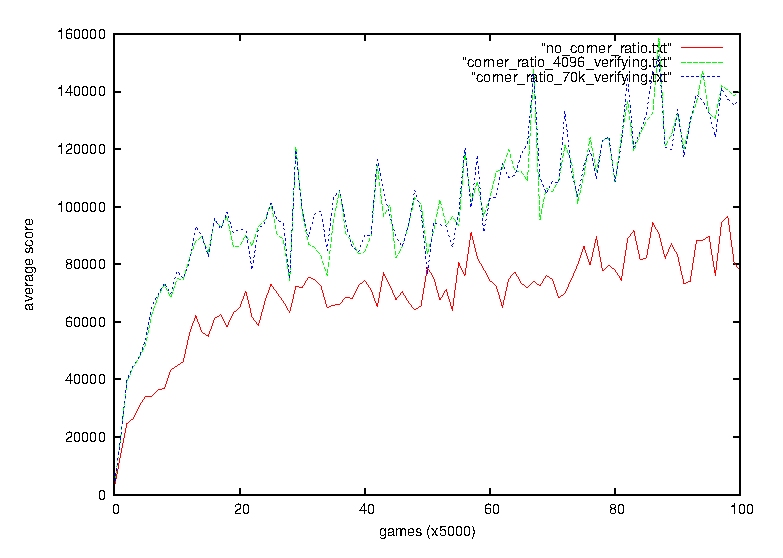
\includegraphics[width=13cm]{figure_007.eps}
	\caption{実験2の結果 - 検証ゲームへのmaximum-in-corner方策の適用}
	\label{figure_007}
	\end{center}
\end{figure}

\begin{figure}[tb]
	\begin{center}
	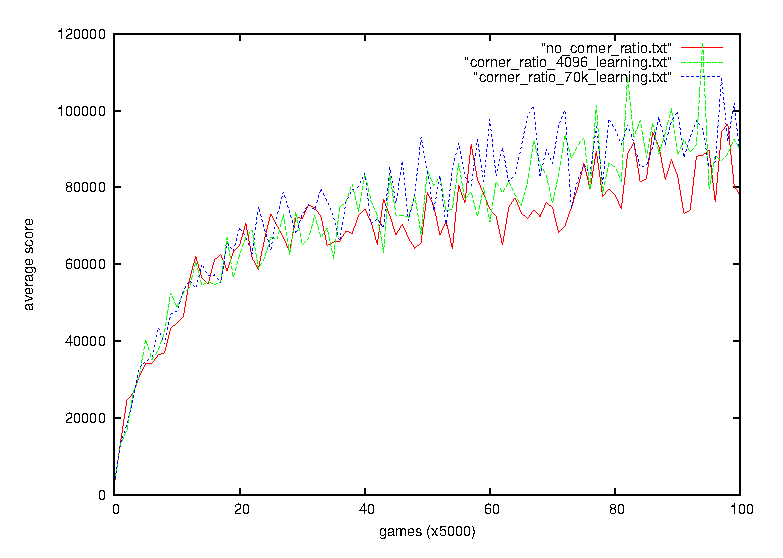
\includegraphics[width=13cm]{figure_008.eps}
	\caption{実験2の結果 - 学習ゲームへのmaximum-in-corner方策の適用}
	\label{figure_008}
	\end{center}
\end{figure}

\begin{figure}[tb]
	\begin{center}
	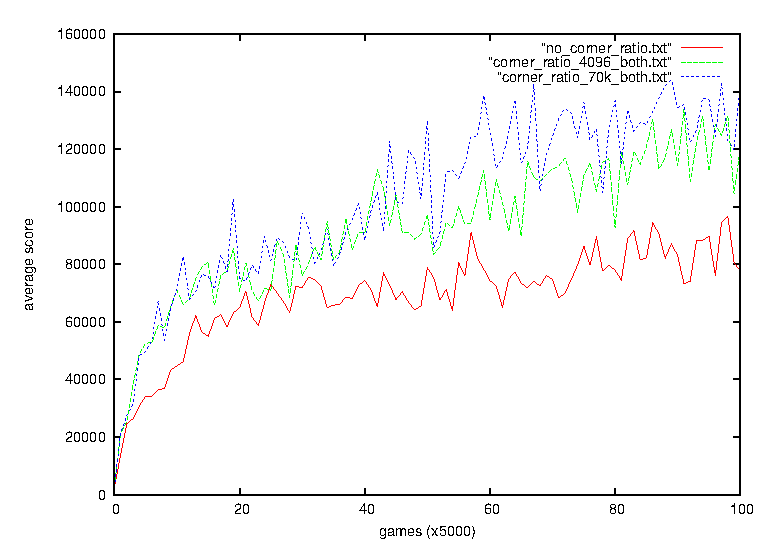
\includegraphics[width=13cm]{figure_009.eps}
	\caption{実験2の結果 - 検証・学習ゲームへのmaximum-in-corner方策の適用}
	\label{figure_009}
	\end{center}
\end{figure}

実験2の結果,ゲームの進行に応じてcorner ratioを変更することにより,TD学習によって学習器の性能が良くなった後でも,maximum-in-corner方策を適用することでさらなる成績の向上が行われることがわかった.それと同時に,ゲームの進行に応じてcorner ratioを割り引くことで,corner誤謬の発生を抑制できるということもわかった.最後に,より適切なcorner ratioの変更の条件を求めつつ,さらに2048プレイヤとしての性能を高めるため,学習率と学習ゲーム数を変更する実験を行った.

\section{実験3:学習率および学習ゲーム数を変更する}
実験3においては,より2048プレイヤとしての性能を高めるために,学習率を0.0025に引き下げ,学習ゲーム数を従来の2倍の1,000,000ゲームに変更した.学習率を引き下げることで価値関数$V$の更新が穏やかになるため,学習の速さは若干遅くなるものの,その分精密な学習がなされて最終的な性能は高くなることが期待される.これに加えて,ゲーム中のスコアに応じてcorner ratioを変更することが有効であると判明した実験2の結果を踏まえて,corner ratioを変更する条件として設定するスコアの境界値をさまざまな値に変動させて実験を行った.その他の条件も含めた実験のセッティングは以下の通り.

\begin{itemize}
\item 学習ゲーム数:1,000,000
\item 学習率:0.0025
\item nタプルネットワークの配置:Wuのスタイル
\item \textsc{ChooseBestTransitionAfterstateCorner}を使用するゲーム\footnote{実験2において学習ゲームのみにChooseBestTransitionAfterstateCornerを使用することには効果が見られないことがわかったため,実験3の条件からは除外した}:
\begin{itemize}
\item 使用しない(ベースライン)
\item 検証ゲーム
\item 検証ゲームと学習ゲームの両方
\end{itemize}
\item 使用するcorner ratio:${\rho}=1.1 \text{もしくは} 1.2$
\item corner ratioを変更する条件:
\begin{itemize}
\item 最初は${\rho}=1.2$とし,スコアが60,000に到達したら${\rho}=1.1$とする
\item 最初は${\rho}=1.2$とし,スコアが70,000に到達したら${\rho}=1.1$とする
\item 最初は${\rho}=1.2$とし,スコアが80,000に到達したら${\rho}=1.1$とする
\end{itemize}
\item ランダムシード:3種類
\end{itemize}

この実験の結果のうち,平均スコアの推移をプロットしたグラフを図\ref{figure_011}から図\ref{figure_013}に示す.ランダムシードによって結果に差があるが,全体的に見て以下の傾向を読み取ることができる.

\begin{figure}[tb]
	\begin{center}
	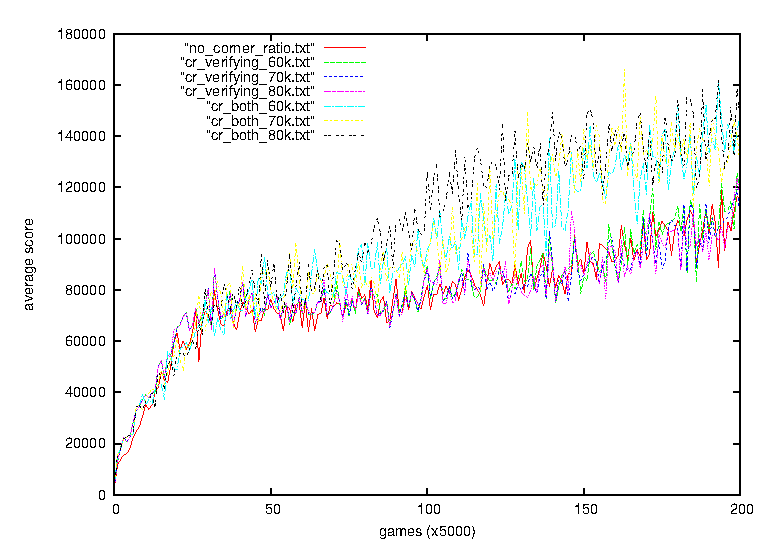
\includegraphics[width=13cm]{figure_011.eps}
	\caption{実験3の結果 - ランダムシードA}
	\label{figure_011}
	\end{center}
\end{figure}

\begin{figure}[tb]
	\begin{center}
	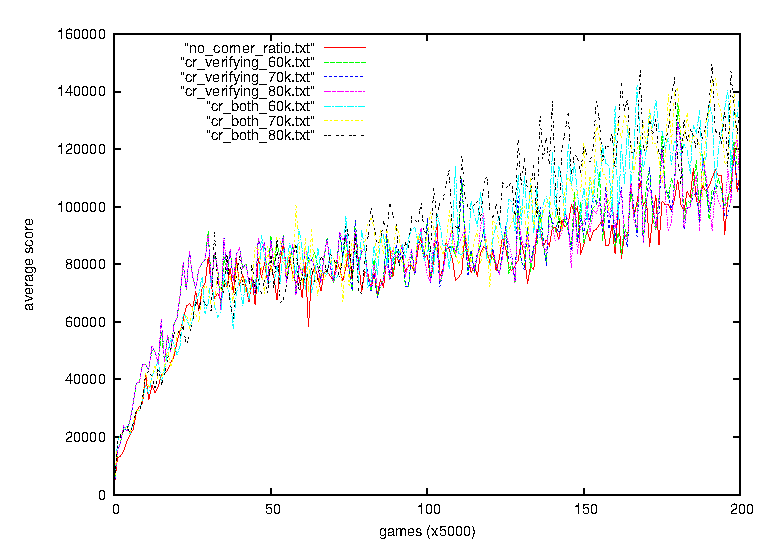
\includegraphics[width=13cm]{figure_012.eps}
	\caption{実験3の結果 - ランダムシードB}
	\label{figure_012}
	\end{center}
\end{figure}

\begin{figure}[tb]
	\begin{center}
	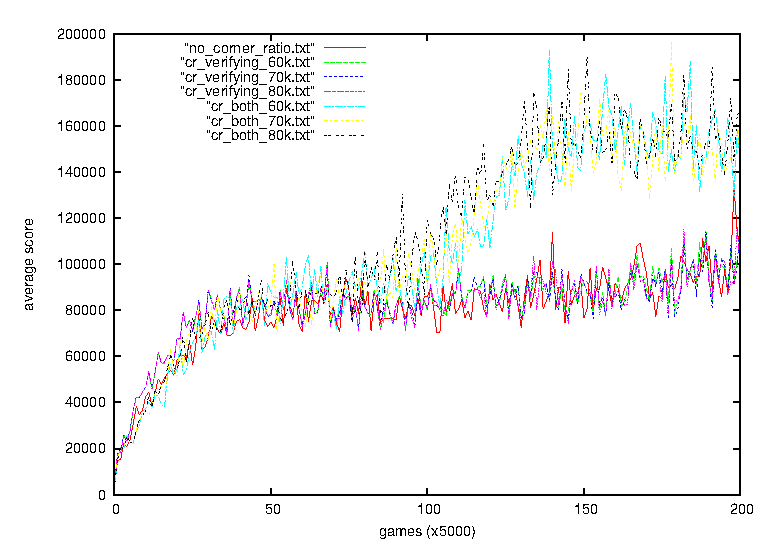
\includegraphics[width=13cm]{figure_013.eps}
	\caption{実験3の結果 - ランダムシードC}
	\label{figure_013}
	\end{center}
\end{figure}

\begin{itemize}
\item 学習率0.0025の条件の下においては,検証ゲームのみにmaximum-in-corner方策を適用しても,ベースラインと比べて顕著な差は現れない
\item 約300,000ゲームほど学習するまでは,どの条件の間にも顕著な差は見られない
\item 約500,000ゲームほど学習した後は,検証ゲームと学習ゲームの両方でmaximum-in-corner方策を適用したプレイヤの性能が顕著に良くなる
\item 局所的に他のプレイヤが上回っていることもあるが,全体的に見ると「検証ゲームと学習ゲームの両方」で「最初は${\rho}=1.2$とし,スコアが80,000に到達したら${\rho}=1.1$とする」条件でcorner ratioを変更するプレイヤの成績が最も良い
\end{itemize}

\chapter{考察と結論}
以上の実験により,maximum-in-corner方策を適用することで,TD学習を用いて訓練した2048プレイヤの成績をさらに改善できるということが示された.このことは「強化学習による訓練ではmaximum-in-corner方策を習得することができない」という2048プレイヤの性質と表裏一体であり,強化学習とは別の観点から2048プレイヤの改良を行えることを示したとも言える.

一方で,maximum-in-corner方策の一面的な導入が必ずしも良い結果をもたらすとは限らないことも示された.常に${\rho}=1.2$としたプレイヤの成績は十分学習されたTD学習のみを用いたプレイヤに劣り,学習が進めば進むほどcorner誤謬が発生する確率も高まることが確認されている.この問題を解決するためにcorner ratioの値を変更することが有効であり,特にゲーム内のスコアに応じてcorner ratioを割引することはプレイヤの成績の改善に大きく貢献した.

しかしながら,本研究において,corner bonusの割引は実験者による手動操作によってのみ行われており,より適切なcorner ratioの選定・決定方法が存在する可能性もある.例えば,Ja\'{s}kowski (2017)によって提案されたTC$({\lambda})$における学習率の自動的な適応のように,ゲーム内のパラメータや指標を参照して,自動的にcorner ratioを決定するといった手法が考えられる.より精密なcorner ratioの追究が不十分であることは,本研究が残した課題の1つである.

maximum-in-corner方策の他にも,2048において人間が経験的に習得しているが,強化学習によるプレイヤが習得できない方策が存在する可能性は少なくないと思われる.強化学習と人間の経験的知識の融合により,2048を始めとするゲームAIエージェントの改良が期待される.

\backmatter
\chapter{謝辞}
本研究を進めるにあたり,1年間ご指導いただき,実験にあたって計算資源を提供していただいた,指導教員の山口和紀教授に感謝いたします.また,Yゼミにて本研究や発表内容に対してアドバイスをくださった山口和紀研究室の皆様にも感謝いたします.最後になりますが,3年次に履修した実習にて,課題として2048プレイヤの作成というテーマを課していただき,本研究の端緒を開いてくださった金子知適准教授に感謝の意を表させていただきます.

\begin{thebibliography}{}
 \bibitem{2048game} 2048. https://gabrielecirulli.github.io/2048/. 2018年1月7日閲覧.
 \bibitem{BusinessInsider} Megan Rose Dickey. Puzzle Game 2048 Will Make You Forget Flappy Bird Ever Existed. Business Insider, https://www.businessinsider.com/2048-puzzle-game-2014-3. 2018年1月7日閲覧.
 \bibitem{CirulliMedium} Gabriele Cirulli. 2048, success and me. https://medium.com/@gabrielecirulli/2048-success-and-me-7dc664f7a9bd. 2018年1月7日閲覧.
 \bibitem{Szubert} Marcin Szubert \& Wojciech Ja\'{s}kowski. Temporal Difference Learning of N-Tuple Networks for the Game 2048. In IEEE Conference on Computational Intelligence and Games, pages 1-8, Dortmund, Aug 2014. IEEE.
 \bibitem{Wu} I-Chen Wu, Kun-Hao Yeh, Chao-Chin Liang, Chia-Chuan Chang, Han Chiang. Multi-Stage Temporal Difference Learning for 2048. In Technologies and Applications of Artificial Intelligence, pp 366-378. Springer, 2014.
 \bibitem{Oka} Kazuto Oka \& Kiminori Matsuzaki. Systematic Selection of N-Tuple Networks for 2048. In International Conference on Computers and Games (CG 2016), Leiden, The Netherlands, 2016.
 \bibitem{Yeh} Kun-Hao Yeh, I-Chen Wu, C. H. Hsueh, Chia-Chuan Chang, Chao-Chin Liang, and Han Chiang. Multi-stage temporal difference learning for 2048-like games. In IEEE Transactions on Computational Intelligence and AI in Games, preprint. 2016.
 \bibitem{Jaskowski} Wojciech Ja\'{s}kowski. Mastering 2048 with Delayed Temporal Coherence Learning, Multi-Stage Weight Promotion, Redundant Encoding and Carousel Shaping. In IEEE Transactions on Computational Intelligence and AI in Games, preprint. 2017.
 \bibitem{Sutton} R. Sutton \& A. Barto.『強化学習』(三上貞芳・皆川雅章訳)森北出版, 2000.
 \bibitem{Tesauro} G. Tesauro. Temporal Difference Learning and TD-Gammon. Communications of the ACM, vol. 38, no. 3, pp. 58-68, 1995.
 \bibitem{Runarsson} T. P. Runarsson \& S. M. Lucas. Co-evolution versus Self-play Temporal Difference Learning for Acquiring Position Evaluation in Small-Board Go. IEEE Transactions on Evolutionary Computation, vol. 9, no. 6, pp. 628-640, 2005.
 \bibitem{Schraudolph} N. N. Schraudolph, P. Dayan, \& T. J. Sejnowski. Learning to Evaluate Go Positions via Temporal Difference Methods. In Computational Intelligence in Games, ser. Studies in Fuzziness and Soft Computing, N. Baba and L. C. Jain, Eds. Springer Verlag, Berlin, 2001, vol. 62, ch. 4, pp. 77-98.
 \bibitem{Dries} S. van den Dries \& M. A. Wiering. "Neural-Fitted TD-Leaf Learning for Playing Othello With Structured Neural Networks. IEEE Transactions on Neural Networks and Learning Systems, vol. 23, no. 11, pp. 1701-1713, 2012.
 \bibitem{SzubertOthello} M. G. Szubert, W. Ja\'{s}kowski, \& K. Krawiec. On Scalability, Generalization, and Hybridization of Coevolutionary Learning: A Case Study for Othello. IEEE Transactions on Computational Intelligence and Al in Games, vol. 5, no. 3, pp. 214-226, 2013.
 \bibitem{Baxter} J. Baxter, A. Tridgell, \& L. Weaver. Learning to Play Chess Using Temporal Differences. Machine Learning, vol. 40, no. 3, pp. 243-263, 2000.
 \bibitem{Bledsoe} Woodrow Wilson Bledsoe \& Iben Browning. Pattern recognition and reading by machine. In Proc. Eastern Joint Comput. Conf., pages 225–232, 1959.
 \bibitem{Lucas} Simon M. Lucas. Learning to play Othello with N-tuple systems. Australian Journal of Intelligent Information Processing Systems, Special Issue on Game Technology, 9(4):01–20, 2007.
 \bibitem{Bagheri} S Bagheri, M Thill, P Koch, \& W Konen. Online Adaptable Learning Rates for the Game Connect-4. Computational Intelligence and AI in Games, IEEE Transactions on, 8(1):33–42, 2016.
 \bibitem{Mahmood} Ashique Rupam Mahmood, Richard S Sutton, Thomas Degris, and Patrick M Pilarski. Tuning-free step-size adaptation. In Acoustics, Speech and Signal Processing (ICASSP), 2012 IEEE International Conference on, pages 2121–2124. IEEE, 2012.
 \bibitem{IDBD} Richard S Sutton. Adapting bias by gradient descent: An incremental version of delta-bar-delta. In AAAI, pages 171–176, 1992.
\end{thebibliography}

\end{document}
